   
 \chapter{Background}    
 \label{ch:background}  
  This chapter introduces the necessary theoretical background for the rest of the dissertation. First, we introduce autonomic computing and adaptive systems. These are explained in the context of the MAPE-K loop, a guideline for designing autonomic systems.  
  %that suggests the integration of a monitoring systems, analyzers, planners, and execution engines.      
  We also introduce some necessary components from control theory. We review optimal linearized control, policy iteration, sub-optimal heuristic control, steady-state equivalent problems and model predictive control (MPC) as different ways to construct control loops. Finally, we introduce Layered Queuing Models (LQM) as a tool to model the performance of clouds. We also provide an explanation about the way we map the cloud concepts (i.e. end-users, services and invocations, infrastructure, and replication) to the model elements (i.e. user classes, delay and queuing centers, and service demands, etc.).  We then review the solution techniques for the closed queuing networks considering software contention and multiple resources. 
   
 \section{Elements of Autonomic Computing and Adaptive Systems}
  Autonomic computing, a term introduced by IBM~\cite{computing2005architectural}, relates to systems that are self-managing, self-tuning, self-healing, self-protecting, self-adapting, self-configuring, and self-organizing (briefly called self-* systems) \cite{babaoglu2005grassroots}. 
Some examples of IT\nomenclature[A]{IT}{Information Technology} related self-* areas of research are:
adaptive parameter-level configuration management \cite{ensink2004coordinating, chang2000automatic, cangussu2004control},  
adaptive client-server communication \cite{loyall1998specifying, noble1997agile, balan2003tactics},  
adaptive resource allocation \cite{doyle_model-based_2003,lee1999scalable}, 
self-configuring network services \cite{huang2004building}, 
workload adaptive services \cite{menasce-accessing-ICAC-2004}, 
self-managing storage \cite{mesnier2004file}, 
statistical inference based decision-making management \cite{cohen2004correlating}, and change and configuration management \cite{wang2003strider}.  

 The autonomic computing subspecialty relevant to this work is the building of self-optimizing complex resource sharing systems that manage themselves in accordance with specific high-level objectives~\cite{kephart_vision_2003}. The autonomic aspect focuses on the fact that the management is performed by the systems themselves rather than being actively performed by human operators. This management is to be in accordance with system management objective set by administrators. An autonomic manager typically understands the desired system objectives, matches those objectives with the current or forecasted system behaviour, and incorporates the objectives into its decisions governing the system. 

  There are options in considering autonomic management system architecture.
 In the architecture considered in this research, adaptation strategies and mechanisms are separated from the applications or systems \cite{garlan2004rainbow, tesauro_utility_2004}. 
The architecture used is the well-known Monitor-Analyze-Plan-Execute (MAPE)\nomenclature[A]{MAPE}{Monitor-Analyze-Plan-Execute}  loop suggested by IBM~\cite{computing2005architectural}, where several components such as an analyzer, automated learner, forecaster, and a planner are used to decide proper actuator action(s) given the current system measures. Figure \ref{fig:mapeloop}, adopted from \cite{mape-loop-pic}, presents a schematic structure of such loop.
\begin{figure}[h]
	\centering		
	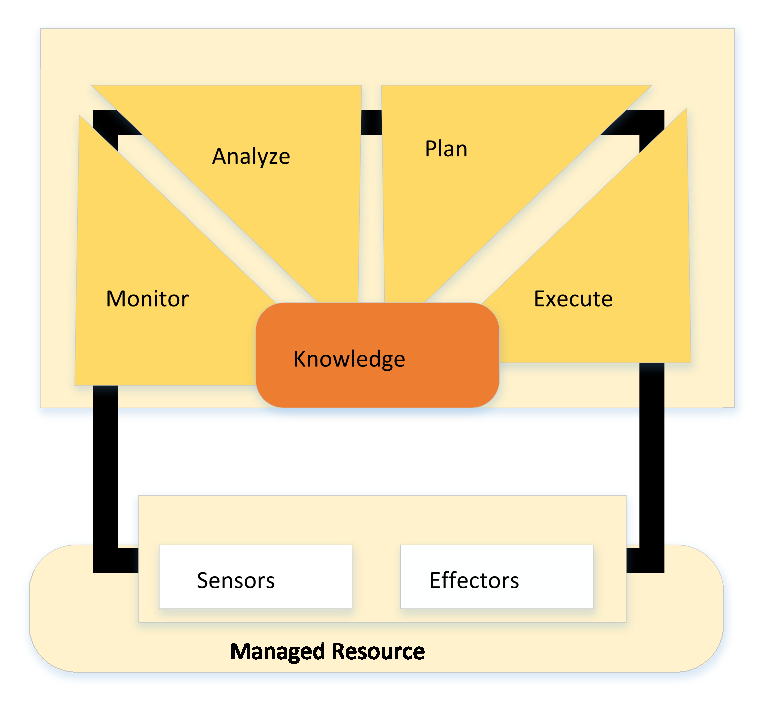
\includegraphics[width=0.45\textwidth]{image/mapeloop1.eps} 
	\caption[Architecture of autonomic management loop.]{Architecture of autonomic management loop suggested by IBM (adopted from \cite{mape-loop-pic}).} 
	\label{fig:mapeloop}
\end{figure}
  
 Components of the autonomic loop have a specific interpretation when viewed in the control theory context. 
 The following is an enumeration (description) of autonomic loop components considering control theory.
 % Below, we enumerate components of the autonomic loop and describe them in the context of the control theory. % Figure \ref{fig:control-loop} presents a schematic structure of such control loop.
 In a control theory sense, the goal of any optimal control loop is to choose a sequence of feasible \textit{control actions} over time that maximize a defined \textit{performance criterion} (or objective function)\footnote{One can instead say the optimal control minimizes an expected total cost function.}.


 \subsection{Monitoring Subsystem} The monitoring subsystem is responsible for measuring inputs, and outputs of the managed system (system I/O in a control theory sense), quantifying system I/O, sometimes aggregating system I/O, and keeping system I/O as a history. In a closed-loop (or feedback based) control, the controller constantly considers the most recent monitored data for calculating the proper actions. 

 Several computer system performance metrics can be collected. For example, hardware level metrics for each host, operating system metrics (e.g. file, network, and memory management subsystems), process level metrics, and service specific metrics for specific types of server processes (e.g. load balancer, web server, application server, and the database server). In a batch-oriented system there are additional metrics, such as the average number of jobs in a queue or the average job's queuing time. There are existing tools for monitoring computer systems, such as
 \textit{Collectd}~\cite{collectd}, \textit{Nagios}~\cite{nagios}, Java Management Extensions (JMX)~\cite{jmx}\nomenclature[A]{JMX}{Java Management Extensions}, and IBM Tivoli monitoring\cite{ibm_tivoli_monitoring}. 
  
   \subsection{Analyzer}
    The analyzer subsystem of the autonomic management loop, identifies and tunes a model of the system, and estimates the unobservable portion of the system state. The model enables the autonomic manager to project the system's behaviour and the state, from the current state under different actions.  A major concern is the ability to synchronize the model based on observed behaviour of the system. In our case, the analyzer is composed of a first principle mathematical model encoding the system's knowledge combined with statistical techniques to perform data-driven learning. 

 \subsection{Planner} 
 A planner uses the model to rapidly explore multiple decisions and find near-optimal solution \cite{litoiu_hierarchical_2005,aiber2004autonomic}. The search space is formed by the actions over time. The search for finding the proper actions can be based on a mathematical optimization in continuous space (e.g. methods such as primal decomposition, interior point methods, stimulated annealing, etc.) or can be a search in the discrete space (e.g. a combinatorial optimization).
  Whether the search is continuous or discrete, it is directed towards a goal or a set of goals.

\section{Optimal Control Theory}  
  In general, the goal of any optimal control approach is to choose the sequence of feasible control actions that maximizes a defined performance criterion (or an objective function) of the following form: 
 \begin{align}
   & \underset{u_0,...,u_{T-1}} {\text{minimize  } }  \lim_{T\to\infty}  \frac{1}{T} E\left[\sum_{t=0}^{T-1} g(x_t,u_t) \right]   \label{eq:general-control-problem-1} \\ 
   & x_{t+1}=f(x_t,u_t)+w_t  \label{eq:general-control-problem-2} \\ 
   & h(x_t,u_t)  < 0 \label{eq:general-control-problem-3} 
  \end{align}
  
  where $x_t$ is the system state,
  $E[\ldots]$ denotes the expected value,  
  $u_t$ is the controlled input, 
  $w_t$ is the uncontrolled stochastic input, 
  $T$ is the control interval, 
  $g$ is the (non)linear stage cost function, 
  $f$ is the (non)linear state transition function which maps the current state to the next one,   
  $h$ is the nonlinear function defining the limits of possible inputs and states.      
  Equation \ref{eq:general-control-problem-1} denotes that the objective is to minimize the overall cost, from the current time step to infinity (i.e. infinite horizon control), by choosing the optimal control inputs. The equation \ref{eq:general-control-problem-2} is called the process model and determines how the system state moves from one step to the next. 
  The inequality \ref{eq:general-control-problem-3} defines a set of possible state-input combinations at any given time. For example, if at state $x_1$ input $u_1$ is allowed, then $(u_1,x_1)$  will be in the set representing the $h$.   
  
In a feedback based scheme or a \textbf{closed loop control}, at any given time, the controller makes its decisions (i.e., to allocate resources) based on the information available from the system up to that time. % and the information deduced and maintained by the controller itself.  
   The solution to the above optimization is obtained and applied at each step of the control. Thus, the original plan is adjusted according to the new observation samples of the environment from the previous step. This solution is called a control policy: 
  \begin{align}
  \phi_t=\mathbf{R^{(t+1)n}}\to \mathbf{R^{m}}   \nonumber \\ 
  u_t=\phi_t(x_0,...,x_t) \nonumber
  \end{align}
  where $n$ is the number of the state variables, $m$ is the number of the input variables, and $t$ is the index of the current time step.

Normally for solving this optimal control problem one must form a set of equations according to dynamic programming principles. For most cases, the dynamic programming is often quite challenging and impossible for large problems. 
%\begin{figure}[htbp]
%\begin{center}
%% \includegraphics{figure/global_view1} 
%\caption{default}
%\label{default}
%\end{center}
%\end{figure}
In the following subsections, we briefly summarize those control problems of interest that can be solved analytically or computed numerically with polynomial complexity. These control problems include linearized dynamic control, optimal linearized dynamic control, policy iteration in finite state models, heuristic policies, and model predictive control (MPC).   
 The proposed controllers vary in their architectural complexity; which depends on the existence of a model for the target system, the theory underpinning the model, and the usage (or omission) of an estimator to track hidden variables in the model. 

\subsection{Optimal Linearized Control}
\label{sec:optimal-linearized-control}       
In some control problems, the optimal control policy has static state feedback control form: $u_t=\psi_t(x_t)$. Using this policy, an optimal input at every step can be obtained from the current state (as opposed to the current and previous states $u_t=\phi_t(x_0,...,x_t)$). 
 For example, consider the Linear-Quadratic-Gaussian (LQG)\nomenclature[A]{LQG}{Linear-Quadratic-Gaussian} control problem:
 \begin{align}
   & \underset{u_0,...,u_{T-1}} {\text{minimize  } }   \lim_{T\to\infty}  \frac{1}{T} E\left[\sum_{t=0}^{T-1} l(x_t,u_t)\right]   \label{eq:linear-control-problem-1} \\  
   & x_{t+1}=Ax_t+Bu_t+w_t \label{eq:linear-control-problem-2} \\ 
   &  F_x x_t + F_u u_t < f  \label{eq:linear-control-problem-3}      
  \end{align} 
   Here the symbols $x_t$, $u_t$, $w_t$, $T$ have the same meaning as equations \ref{eq:general-control-problem-1} to \ref{eq:general-control-problem-3}; they subsequently denote the system state, control input, stochastic input, and system lifetime. 
   $l$ denotes the Euclidean (or second) norm function (i.e. $\|\boldsymbol{x}\| := \sqrt{x_1^2 + \cdots + x_n^2}$). 
$F_x$  and $F_u$ are convex functions of $x$ and $u$.
$f$  is a convex function.
Finally, $A$ and $B$ are matrices.  

The equation \ref{eq:linear-control-problem-1} denotes that the objective is to minimize the overall cost from the current time step to infinity (i.e. infinite horizon control), by choosing the optimal control inputs.  The only difference with \ref{eq:general-control-problem-1} is that here the stage cost function $l$ is quadratic.
Note that, the process model denoted by the equation \ref{eq:linear-control-problem-2}   has a linear form. Also note that, the set of possible state-input combinations, defined by the inequality constraint \ref{eq:linear-control-problem-3}, is guaranteed to be convex. 
  
 The solution (i.e. the control signal) for this problem, has a feedback form, and is itself a linear system called Linear Quadratic Regulator\cite{lqr}. It takes the output of the system under control ($y_t$) as input and generates the proper input to be applied to the system ($u_t$). 
% \hat_{x}=[A-LC-(B-LD)K]\hat_{x}+Ly
% u=-K\hat_{x}
% or 
% in discrete time you just get x and apply this on it 
 Internally, this controller is based on a dynamically adjusted LQ-optimal gain applied on the \textit{state estimate} driven from an estimator. 
 % in discrete time http://www.mathworks.com/help/control/ref/dlqr.html 
 The estimator in LQG is usually a simple or an extended Kalman filter~\cite{welch_introduction_1995} \nomenclature[A]{EKF}{Extended Kalman Filter} able to maintain a good estimate of model unknowns by calibrating itself to measurements during runtime.
 Note that the LQG solution is only optimal for the linear dynamic systems with Gaussian noise, quadratic objectives and no constraints. 
   
   % In this solution, function $mu$, which maps every state to an optimal action, is identified by a LQ\nomenclature[A]{LQ}{Linear Quadratic.} optimal gain and is obtained by directly solving the associated Riccatti equation. 

\subsection{Policy Iteration}  
When the model underlying the system is Markovian with finite states $X$, the problem of finding an optimal policy that maximizes a long-term cost function, has a solution; investigated under the umbrella of Markov Decision Processes (MDP)\nomenclature[A]{MDP}{Markov Decision Process}. 
Computing the optimal value function and policy requires solving a nonlinear system of equations. When the underlying state of the system is hidden (Hidden Markov Model or HMM)\nomenclature[A]{HMM}{Hidden Markov Model}, which is usually the case, solving the problem is not quite so simple. The solution can then be investigated as a Partially Observable Markov Decision Process (POMDP)\nomenclature[A]{POMDP}{Partially Observable Markov Decision Process}. Unlike LQG, in a POMDP, there is no separation principle. Meaning that, one cannot estimate the state distribution and perform optimal control on the known state.\footnote{In LQG the state distribution is Gaussian, and thus, the mean value can be easily used for projecting to future.}
 The solution, in this case, is to pick a policy format and gradually improve the stationary policy using the observed result of the controller. The \textit{policy iteration algorithm} generates a sequence of improving stationary policies. Similarly, the \textit{value iteration algorithm} is then used to converge iteratively towards an optimal cost $J^*$. 
 
 \subsection{Sub-optimal Control}
 There is a small set of problems for which the optimal control policy with a feedback control form can be computed.  However, sub-optimal feedback solutions are extremely common. 
  For example, consider a linear system which is mathematically modelled as: 
  \[ x_{t + 1} = Ax_{t} + Bu_{t} \] 
  where $u_{t'}$ are the control inputs and $x_{t'}$ is the system state. 
  In the \textit{linearized dynamic control}, one should suggest a small or efficient set of control inputs $u$ that transfers $x$ to $x_\text{target}$. %considers the 'state transfer' of a linear system    
 Similarly, a regulation problem involves taking the system output ($y_t$) to a reference output or a set-point ($y_\text{target}$). Assuming the control error is the difference between the current system output and the desired output ($y_\text{target}$): $e_t=y_t-y_\text{target}$, it is desired that control error be transferred to zero.
  % A proper control signal (here allocation actions) is calculated based on control error, where  
        
  A feedback loop for this purpose can be constructed by feeding back the control error (the difference between a set-point and a measured output) as an input to the system (often with some intermediate processing). 
For a system whose dynamics are known
\footnote{The dynamics of a system can be represented in several mathematical forms such as transfer functions, state-space models, difference equations, etc. Depending on the form used, the controller might be designed using the same mathematical method (e.g. a transfer function).}(e.g. through system identification techniques), a proper feedback based regulator can be designed to make the system output achieve a degree of the following properties:  
(i) responsiveness to an error, 
(ii) the degree to which it overshoots the set-point, 
(iii) the degree of oscillation. 
    
For a system whose dynamics are known (e.g. through system identification techniques), a proper controller can be designed using the design techniques such as pole placement, root locus, etc. The model used during system identification can take several forms such as transfer functions, state-space models, difference equations, etc.
 
%\subsection{Steady-State Equivalent Problem} 
%Sometimes the optimal control problem can be converted into a deterministic optimization based on system's steady-state behaviour. In this case, a new \textbf{steady-state equivalent problem} is constructed and solved.   A steady state equivalent problem can be obtained by substituting mean-values with the same $f$ regardless of time index. 
%For example, in case of LQG (equations \ref{eq:linear-control-problem-1} to \ref{eq:linear-control-problem-3}), steady-state equivalent problem is as follows: 
%  \begin{align}  
%   & \underset{\bar{u}} {\text{minimize  } }  l(\bar{x},\bar{u}) \\
%   & \bar{x}=A\bar{x}+B\bar{u}+\bar{w} \\ 
%   & F_x \bar{x} + F_u \bar{u} < f
%  \end{align}
% variables $x_t$ and $u_t$ are considered to have constant values denoted by $\bar{u}$ and $\bar{x}$ and the process noise $w_t$ is considered to have a constant value equal to its mean $\bar{w}$. 
%
%   In the general case of control problems (i.e.  equations \ref{eq:general-control-problem-1} to \ref{eq:general-control-problem-3} ),  the problem has to have certain properties  in order to be   transformed into an equivalent steady-state  form; for example, when $w_t$ is separable from process dynamics and system inputs (i.e. $x_t=f(x_t,u_t)+w_t$) and noise has a certain distribution. 
%  % Note that the structure of $f$ is preserved. 
%
 \subsection{Model Predictive Control (MPC)} 
In Model Predictive Control (MPC) (also referred to as Limited Lookahead Control or LLC)\cite{abdelwahed2004control, kandasamy2004self}\nomenclature[A]{LLC}{Limited Lookahead Control}, the controller explores a search space formed by different choices of control actions over a predicted model \cite{bhat2006enabling} to find an optimal solution; thus, a management problem is posed as a sequential optimization under uncertainty. 
The search space includes a set of future states within a lookahead horizon. Controller then selects a path that minimizes a cumulative cost while satisfying both state and input constraints within the lookahead horizon
$u^*_j|j\in [t , t + N-1]$. 

In a Certainly Equivalent Controller (CEC) implementation, at each time step $t$, one
 makes a set of forecasts $\hat{w}_{t|t} ,\ldots,\hat{w}_{t+N-1|t}$ for future steps based on the observed state trajectory $x_{0},...,x_{t}$. 
% in fact, the only way in which capital Xt comes into this is through $\hat{w}_{j|t}$
 % the observed state trajectory $x_{0},...,x_{t}$ is irrelevant, except in $x_{j+1}$. 
 Then one is simply going to use these forecasts in the following optimal control problem as if the forecast were perfect. The first control input leading to this path is chosen as the next control action.
\begin{align} 
    \underset{u_t,...,u_{N+t-1}} {\text{minimize } }  &  \sum_{j=t}^{t+N-1} l_t(x_j,u_j) + l_{t+N}(x_T)  \label{eq:mpc-control-problem-1}   \\ 
    \text{subject to: } 
    & x_{j+1}=A x_{j}+B u_j + \hat{w}_{j|t} & j=t...t+N-1  \label{eq:mpc-control-problem-2}   \\
    & u_j\in U_j   & j=t...t+N-1  \label{eq:mpc-control-problem-3}  
\end{align}        
 Here $u_t,\ldots,u_{N+t-1}$ are variables and $x_t, \hat{w}_{t|t} ,\ldots,\hat{w}_{t+N-1|t} $  is the known data. The symbol $x_t$ has the same meaning as equations  \ref{eq:linear-control-problem-1}  to \ref{eq:linear-control-problem-3}; it denotes system state at time $t$. $N$ is the length of the lookahead window, $\hat{w}_{j|t}$  is the prediction of future disturbance $w_{j}$ at time $j$. $u_j$ is the future control input at time step $j$. $l_t(x_j,u_j)$ is a quadratic function representing the stage cost at time step $t$. $l_{t+N}(x_T)$ is the cost of deviation of the terminating state $x_T$. $U_j$ is the input constraint at future time $j$.  

 There is a common misconception about model predictive control, that the quality of the derived control inputs only depends on the quality of the predictions.  However, this is not true. In MPC, one forms a prediction of what the future disturbances $\hat{w}_{t|t} ,\ldots,\hat{w}_{t+N-1|t}$ are going to be, based on the observed state trajectory $x_{0},...,x_{t}$. These predictions can be just the mean value of the disturbance (i.e. as opposed to conditional expectation), or they can come from an external analyst. No assumption regarding the correctness of the forecasts is necessary for CEC to work.  In most cases, not one of the $\hat{w}_{j|t}$ will actually come true; despite this, the approach works very well in practice. In fact, if all $\hat{w}_{j|t}$ were true, then the problem would be a deterministic optimal control (as opposed to stochastic control problem). %  while reducing the cost of solving such  stochastic model predictive control problems, to linear with the horizon size.  


%  \subsection{Emergent Behaviour}   
% In \textit{Emergent Behaviour Approach}, autonomic systems can be built based on naturally occurring emergent systems (e.g. flocking\cite{spector2003emergence}, ant colonies \cite{camorlinga2004emergent}, and market economy \cite{kephart2001software,tesauro_utility_2004,eymann2003self}). Complicated patterns can emerge from the interplay large number of autonomous entities that behave according to some simple rules \cite{turing1952chemical, gierer1972theory}. Feedback and reconfiguration can be done in these systems by incorporating evolution through the concept of death or failure (cells die, market actors loose money).  
%
%
% As an example of these systems, virtual markets, composed of numerous simple actors interacting with money, can be used to build complex goal-oriented decision support systems \cite{cheliotis2003autonomic}. For example, in a resource allocation problem in grid infrastructure \cite{foster1997globus,foster2002grid} market-based control can be applied to remove unwanted resource contention. \cite{montresor2003messor} showed how an ant algorithm could be used to solve the problem of dispersing tasks uniformly over a network. Similarly, the Routing Information Protocol (RIP)\nomenclature[A]{RIP}{Routing Information Protocol})  routing table update protocol uses simple local rules that result in good overall routing behaviour. Other examples include autonomous grid scheduling protocols \cite{kreaseck2003autonomous} and peer-to-peer file sharing networks [gnutella, stoica2001chord].  In all of these systems the whole has a functionality more than the sum of the parts.

%
% Assume the Grid manager has to decide about the hosts that should handle tasks based on the resources left on the host (i.e. central processing unit (CPU), network and disk interfaces, and data storage) and the nature of the tasks. In market-oriented approach, one can assign tasks to autonomous entities and letting these entities find a suitable host. Autonomous entities have to use electronic currency to purchase the resources necessary to complete its task. Based on the resource usage at hosts, market determines prices for that host (i.e. congestion results in high prices). Less congestion through even spatial distribution of agents will follow naturally as agents choose hosts with lower prices. Temporal load balancing will be also resulted from the fact that some agents wait until prices drop. 
%


   \section{Cloud Computing}
   % \section{Service Center as a Queuing Network}    
 A Large Scale Software Center (LSSC)\nomenclature[A]{LSSC}{Large Scale Software Center} aims at large scale delivery of on-demand computational power (specifically network storage, computational devices, and services) to a user community.   
 \footnote{Ultra Large Scale systems (ULS)\nomenclature[A]{ULS}{Ultra Large Scale systems}, is a closely related term coined by researchers at Carnegie Mellon's Software Engineering Institute, referring to a system composed of a large set of systems with a variety of stakeholders communicating and operating to satisfy separate (possibly conflicting) goals.}
Current examples of such system include grid computing~\cite{foster1997globus,foster2002grid} and cloud computing~\cite{BHayesACMComm2008,MArmbrustEtAlTR2009,BRochwergerEtALIBM2009,RBuyyaEtAlFGCS2009}. 
    
Grid computing, having arisen from the high-performance computing (HPC)\nomenclature[A]{HPC}{high performance computing}  community near 2000, targets the delivery of on-demand computational power using a unified network of loosely coupled computers in the form of ``super virtual computer". The aim of designers was to let users plug their own programs into the infrastructure, and use resources for a desired duration. 
Current implementations of computing grids usually target long-running resource intensive applications (or jobs) that are submitted by a few users. Examples of these applications are distributed simulation \cite{ddsos,ddsos2},
scientific visualization \cite{wolf2002smartpointers}, 
continual queries \cite{babu2001continuous,kumar2005resource}, 
video conferencing \cite{huang2003network}, 
and transcoding \cite{radiantGrid}.  

Cloud computing is another manifestation of LSSC that, according to many, has caught on in mainstream enterprises.
In the cloud, there is usually a clear distinction between a provider and a customer, and the extent of sharing is governed by economic rules and pricing (usually pay-as-you-go). 
In cloud computing, large condensed data centers, possibly operated by multiple stakeholders, are offered at different levels of abstraction (e.g. infrastructure (IaaS), platform (PaaS) and software (SaaS)) on-demand as commodities to a large community of users. While IaaS focuses on offering virtualized hardware, PaaS hosts applications composed of services, which make use of other infrastructure services. In PaaS, usually a specific programming language and API for infrastructure services is enforced. 
In SaaS, there is a more customized set of APIs for specific types of applications (for example, accounting), shared by all applications of that type. 
 
  The cloud model we consider in this thesis is composed of a set of applications, offering services that are used by end-users. The end-users are usually service consumers around the globe accessing the services through Internet Protocol (IP), and most often Hypertext Transfer Protocol (HTTP). End-users, in our cloud model, are divided into a set of classes, where each class has a certain population and behaviour (in terms of accessing the cloud resources).
  The services are either generic and offered by the cloud provider (such as naming, storage, etc.) or application-specific and developed by cloud consumers. Both services are hosted and administered on the available infrastructure. % The multiplicity of application services is a lot more than the cloud services. 
 Some services developed by the consumers are frontend, meaning that they are the first point of interaction with the end-user, other services are backend, meaning that they are invoked by frontend services.   
  
     In our cloud model, the relationship between classes and applications is one-to-one:  (i) each class uses the limited set of services offered by a single application (ii) there is only one class of users associated with each application.  
     Thus, in this thesis, we can use the concepts of an application and class of users interchangeably. 
    
\section{Service Centers as a Layered Queuing Models (LQM)}  
\label{sec:layered-queuing-models-introduction}   
Queuing theory based models \cite{petriu_approximate_1994,petriu_approximate_2004,badidi-queuing-2005} and Layered Queuing Models (LQM) \cite{rolia_method_1995,ramesh_multi-layer_1998} developed upon Mean Value Analysis (MVA)\nomenclature[A]{MVA}{Mean Value Analysis} of queuing networks have been used to capture the behaviour of multi-tier distributed applications \cite{litoiu_hierarchical_2005, xu_performance_2006,hamoun_ghanbari_tuning,liu_layered_????}. 
Queuing Models can be utilized to describe the expected performance of service centers (i.e. response time and throughput) in relation to various inputs. In the following subsections, we review the components of the queuing models.  

\subsection{Workload} 
\label{sec:workload-background}  
  In this section, we review workload parameters derived from a workload characterization, including workload intensities and service demands.    
 
 \subsubsection{Workload  Intensities}  
 \label{sec:workload-intensities-background}  
 Software components hosted in the cloud can be categorized %from workload point of view into services and standalone programs. 
 Workload of a service is driven by its external users but workload of a standalone software component (such as a simulator or a batch data processor) is controlled by itself or its data.  
 Both types of software components can be generalized as one. 
 In the first case, the workload is specified as a \textit{number of users} or a \textit{request rate}, and in the second case it is usually specified as a \textit{multiprogramming level} (the number of simultaneous threads running on behalf of a process) or an \textit{execution frequency} (the frequency that a specific software module is called).   
 The number of users for a service is equivalent to the multi-programming level and the user request rate is equivalent to the execution frequency.
   
 In general, the workload component can be modelled as either {\it closed} or {\it open}. In the open model, customers are assumed to make requests on average every $\tau$ seconds, independent of when they receive responses for the previous requests. The open workloads are identified by an average request inter-arrival time ($\tau$)\nomenclature[M]{$\tau$}{Workload's average request inter-arrival time}, which is measured in seconds, or an arrival rate ($\lambda$)\nomenclature[M]{$\lambda$}{Workload's average request arrival rate}, which is measured in requests per seconds. Often, these models assume that the arrival rate ($\lambda $) is a homogeneous Poisson process, and that inter-arrival times ($\tau $) are exponentially distributed with parameter $\lambda $ (mean of 1/$\lambda $).  
In a closed model, clients are assumed to wait for responses to their requests.  Upon receipt of this response, the client spends some time determining the next action before issuing a further request. Closed models are defined by the number of users ($N$\nomenclature[M]{$N$}{Workload's average number of total users}) and average think time ($Z$\nomenclature[M]{$Z$}{Workload's average customer think time}). The think time is considered to have an exponential distribution.

A service center may offer a large number of services where each service is used by more than one group of users. Each group of users may consume the services and the resources in a different way (for example, with highly different CPU demands). Thus, it is common to refer to each group as a different \textbf{class}. In multi-class models, outputs are given in terms of the individual customer classes. It is, therefore, reasonable to model each application with a separate class
of users. In the case of open multi-class models (with say $C$\nomenclature[M]{$C$}{Number of customer classes in the workload} customer classes), workload intensity is denoted by $\lambda\equiv(\lambda_1 \dots \lambda_C)$, where $\lambda_c$, is a class $c$\nomenclature[M]{c}{Index of a customer class} arrival rate. A closed multi-class model consists of $C$ classes, each of which has a fixed population. We denote the workload intensity by $N\equiv(N_1 \dots N_C)$ and by its think time $Z\equiv(Z_1\dots Z_c)$, where $N_c$\nomenclature[M]{$N_c$}{Number of users in class $c$} is the class $c$ population size, and $Z_c$\nomenclature[M]{$Z_c$}{Think time of class $c$} is the class $c$ think time. 

 \subsubsection{Workload demand: Interaction with Resources}  
 \label{sec:workload-demands-background}  
 A service and an application can be modelled by a set of queues, where devices are mapped to queuing or delay centers. CPU is the main resource consumed by programs.  Other resources such as hard disks and network are used from CPU. The programs accessing system resources are modelled as the customers of the queuing network. By modeling the cloud workload as a queuing network model, the general Mean Value Analysis (MVA) can be used to calculate the performance characteristics of the system. 
 
  In queuing models, service interaction with hardware resources is quantified in terms of service times.  The service time $D_{s,k}$\nomenclature[M]{$D_{s,k}$}{Service time of service $s$ at resource $k$ per visit to the service} is the time each request spends on a resource type $k$ when accessing service $s$. 
  For example, \texttt{view cart} service that is executed on an application server could be  characterized by the following  parameters: $D_{\mathtt{view cart},\text{CPU}}=30 \text{ ms}$, $D_{\mathtt{view cart},\text{DISK}}=30 \text{ ms}$. 
  Here, we assume the basic operations performed at the device when executing the service by the various  classes are the  same; thus, it is  reasonable  to  assume  that  the  average  service  times across classes are nearly equal.   
 %% Under common scheduling policies such as first-come-first-served (FCFS) scheduling all customer classes $c$ have
 % In a service-oriented system, the service demand $d_{c,s,k}$\nomenclature[M]{$d_{c,s,k}$}{Service demand of service $s$ of class $c$ at resource $k$ for a single visit to the service.} is the sum of all service times on resource type $k$ during one execution of service $s$ of  class $c$ ; thus it is indexed by the service $s$, the class $c$ and the resource $k$. 
     However, it is possible for different customer classes to require different total numbers of visits to the service center ($V_{c,s}$)\nomenclature[M]{$V_{c,s}$}{The visit ratio of class $c$ to service $s$. Or total direct and indirect mean requests to a service $s$ for one request from a user class $c$}, thus providing distinct service demands (which we denote by $d_{c,s,k}$):
     \begin{align} \label{eq:new-demands} 
       d_{c,s,k}= V_{c,s} D_{s,k} 
     \end{align}
     here $V_{c,s}$ is the \textit{visit ratio} of class $c$ to service $s$. It represents the total direct and indirect mean requests to a service $s$ for one request from a user class $c$\footnote{If $V_{c,s}$ is normalized (i.e. $\sum_s V_{c,s}=1$) then accesses to the $S$ services fall into a distribution referred to as the \textit{Web Interaction Mix}. For example, TPCW benchmark specifies two web interaction mixes: ``One is intended to simulate a workload where there are few buy orders and the majority of the customer requests are browsing the website. This is accomplished by having 95\% of the web pages accessed be the browsing pages, (Home, New Products, Best Sellers, Product Detail and Search pages) while only 5\% of the Web accesses are to the order web pages. This mix tends to place more pressure on the front-end Web Servers, Image Servers and Web Caches. The second mix is intended to simulate a website with a significant percentage of order requests. This is accomplished by having 50\% of the web page accesses be the browsing pages and 50\% of the accesses be to the order web pages. The second mix stresses the Database Server."\cite{tpcw_benchmark}}.  
  $d_{c,s,k}$ is the total service demand the service $s$ makes on a resource $k$
  %  (Possibly by several visits) 
  by a single request of class $c$\nomenclature[M]{$d_{c,s,k}$}{the total service demand made on service $s$, by a single request of class $c$.}. 
 % The actual number of accesses for a customer of each class can be represented in the model by appropriate values of the $V_{c,s}$ for each class $c$. 
 \subsection{Deriving Visit Ratios}    
 For some service-oriented systems, there is a systematic way to calculate  $V_{c,s}$ as follows: $V_{c,s}$ for front-end services can be calculated by Consumer Behaviour Model Graph (CBMG)\nomenclature[A]{CBMG}{Consumer Behaviour Model Graph}\footnote{CBMG is presented as a state transition graph in the workload characterization process.}  \cite{menasce2004composing}. 
    For backend services $V_{c,s}$ are obtained using the visit ratio of front-end services, and \textit{call multiplicities}  on the edges of \textit{service call graph}. 
       %:cite  the paper composing Web services: a QOS view
      A service call graph is an acyclic directed graph where each edge represents the number of calls from a caller service to a callee and each edge is annotated by a call multiplicity. 
    % 
Using the call graph one can calculate the visit ratios.
Let $\servMeanReq_{es}$\nomenclature[M]{$\servMeanReq_{es}$}{Mean requests made directly from any service $e$ to service $s$} be the mean requests made directly (i.e. call multiplicity) from service $e$ to service $s$. 
 Formally, the \textit{visit ratios} satisfy the following equation:  
\[  \left\{ 
  \begin{array}{l l}
   V_{c,s}=\sum_{s'=1}^{S} V_{c,s'} y_{s',s} & \quad \text{where $s$ is a backend service}\\
    V_{c,s''}  \quad \text{is computed from CBMG}, & \quad  \text{where $s''$ is a front end service}
  \end{array} \right.\]

 Algorithmically, $V_{c,s}$ is calculated from the call graph $\servMeanReq_{es}$ using the following set of equations\footnote{Assuming there are no request cycles, $Y_{cs}$.}:  
 % For this purpose user class $c$ will be defined to have an entry numbered S + c, and yS+c,s is the mean number of requests made directly to entry $s$ for one user response. 
%
%setting $Y_{c,S+c} = 1$ for all $c$, and using:    
%$ Y_{c,c+S} ,  Y_{cs} = \sum_{e=1}^{\numService+\numClasses} Y_{ce} y_{es}  $. 
\begin{align} 
& con^0=\zeros_{\numService+\numClasses, \numService+ \numClasses} \label{eq: compute-adjacency-matrix}  \\
& con^{(i)}= con^{(i-1)}+ \servMeanReq^i  \text{ for } i \in 1\ldots \text{levels}   \nonumber \\ 
&V=con^\text{levels}_{1\ldots \numClasses, \numClasses+1\ldots \numClasses+\numService} \nonumber 
\end{align}  
where  $con^{(i)}$ represents the \textit{contact level} of services and classes at the $i$'th iteration, taking $\servMeanReq$ as the adjacency matrix and $\servMeanReq^i$ is the power of $\servMeanReq$, or in simple words it is the contact level of each node to its $i$'th further away node.  
% \textit{contact level} of any front-end service to a backend service. 
For example, if web service B and C provide services to A, and services B and C both use web service E, then the $con^2$ from A to E  is calculated as $y_{AB}y_{BE}+y_{AC}y_{CE}$.  

% The demand of user classes on software-hardware resources is calculated based on usage of the services by user classes, the internal usage of services by other services, and the hardware resource demand of the associated services. The steps for calculation are as follows:
     
 \subsection{Replication} 
 When services are replicated, multiple instances are deployed on multiple hosts. Each replica is indexed by $j=(s,h)$ where $s$ represents the service and $h$ represents the host for the replica. Here the load of the original service is distributed between the replicas.
 One can adjust the load on each replica by distributing the accesses to replicas in a desired proportion. This distribution can be modelled by changing the call multiplicities in the call graph in the edges between the callers and the callee service replicas, or by directly considering the call multiplicities in visit ratios $V_{c,s}$.  
  Note that in case of the replication, service demands between replicas are shifted based on $V$ as the equation \ref{eq:new-demands} can be written as:
  % the sum of visit ratios for replicas of the same service is preserved: 
   \[ d_{c,s,k,h}=  V_{c,s,h} D_{s,k} \] 
   \[V_{c,s} = \sum_h V_{c,s,h} \]
   Also according to \cite{menasce1999methodology} the average service demand for a class $c$ on a resource $k$ of a host $h$ can be obtained from the original service demands as follows: 
    %\[ d_{c,k}=\sum_s d_{c,s,k} \]  
   \[ d_{c,k,h}=\sum_s d_{c,s,k,h} \]  
 % For onote that according to equations ....  this will eventually change that demand on resources. 
 \nomenclature[M]{$d_{c,k,h}$}{The total service demand made by a single request of class $c$ on resource $k$ of host $h$.} 
  Here, it is assumed that service demands are independent of the class of service and the host where the service is deployed. Essentially, it is separating the servers and the resources such as CPU. 
%In this case the total number of visits on each resource type $\sum_{k\in \text{same resource}} V_{c,k}$ and  the service time on each replica $S_{c,k}$
% stays the same.  %(for example v1+v2=110). 
%  however, unless the service times of all the replicas  are identical there is no guarantee that  the total service demand is preserved after reconfiguration; Meaning that there is no  notion of preservation of  service demands.


%  \textbf{service demand itself  can be decomposed to } 
%  \textbf{service times} (S)  for each visit and \textbf{the number of visits} (V)  for each request. In a multi-class model the service time, denoted by $S_{c,k}$, is the average service requirement per visit of class c on resource k. From modeling point of view once a request acquires the resource, it remains at that resource for its service time. 
%  Similarity the service demand, denoted by $D_{c,k} $ is defined as average service requirement per request of class c on resource k.  Following relationship holds between the service demand and service time:$D_{c,k} = V_{c,k} S_{c,k}$,  where  $V_{c,k}$ denotes the number of visits per request of class c at resource K. Also throughput of class c at center k is defined as: $X_{c,k}=\lambda_c V_{c,k}$.
% 
% As an example if we observe a system for 8 minutes, and 160 requests of class c are handled during this interval, and the resource k has been busy in total for 2 minutes to handle class c request then the service demand is $D_{c,k}=2*60/160=0.75$. 
%and if 400 visits has occurred for class c requests to resource k, then $D_{c,k}=2*60/400=0.3$. 
%
%In this type of formulation two things are important: 
%1st,  is one wants to project the behaviour of the system to a configuration that resource K is substituted with a faster one, he can divide the service demand of all the classes on that resource  by the factor that the speed is increased.  
% 2nd,  


  \subsection{Solution Techniques for the Closed Queuing Networks }   
 % For example, algorithm \ref{algorithm-open-queuing-solution}, adopted from \cite{lazowska_quantitative_1984}, represents such solution for open model workloads on a flat queuing network.  
 The set of equations giving the mean value analysis (MVA) solution to the model for closed workloads is as follows: 
\begin{align} 
& X_c(\vec{N})=N_c(\vec{N})/(Z_c+\sum_{k=1}^K R_{c,k}(\vec{N})) \label{eq:queuing-model1} \\
& Q_{c,k}(\vec{N})=X_c(\vec{N}) R_{c,k}(\vec{N}) \label{eq:queuing-model2} \\
& R_{c,k}(\vec{N}) = \frac{D_{c,k}}{\speedFactor_k} (1+Q_k(\overrightarrow{N-1_c})) \label{eq:queuing-model3} \\
& Q_k(\vec{N})=\sum_{c=1}^{C} Q_{c,k}(\vec{N})  \label{eq:queuing-model4}  
\end{align}  
 \nomenclature[M]{$X_c(\vec{N})$}{Average system throughput for class $c$ customers for workload $\vec{N}$} 
  \nomenclature[M]{$R_{c,k}(\vec{N})$}{Average delay for class $c$ customer at center $k$ for workload $\vec{N}$} 
   \nomenclature[M]{$Q_{c,k}(\vec{N})$}{Average number of class $c$ requests in resource queue $k$ for workload $\vec{N}$} 
    \nomenclature[M]{$Q_k(\overrightarrow{N-1_c})$}{Total queue length of resource $k$for predecessor workloads $\vec{N-1_c}$ with one class $c$ customer less than $\vec{N}$.}
    \nomenclature[M]{$\speedFactor_k$}{The speed factor of resource $k$} 
    Here, $X_c(\vec{N})$ denotes the average system throughput for the class $c$ customers for the workload $\vec{N}$.
  $R_{c,k}(\vec{N})$ denotes the average delay for the class $c$ customer at the center $k$ for workload $\vec{N}$.
   $Q_{c,k}(\vec{N})$ denotes average number of requests of the class $c$ in the queue of the resource $k$ for the workload $\vec{N}$.
    $Q_k(\overrightarrow{N-1_c})$ is the total queue length of the resource $k$ for the predecessor workloads $\overrightarrow{N-1_c}$ with one class $c$ customer less than $\vec{N}$. 
 $\speedFactor_k$ denotes the \textit{speed factor} of the resource $k$. 
 Here, the speed factor is used to standardize different resources in terms of the speed. This is to make the demands machine and application independent. Demand is described in terms of number of compute seconds for a standard CPU. Transferring a class's workload to different resources is assumed to preserve the standardized resource demand, although the final demand on the resource (i.e. $\frac{D_{c,k}}{\speedFactor_k}$) would depend on the resource's speed factor.  
% CPU work and call this the standard cycle. For example: a single clock cycle on one type of machine might do 1.1 standard cycles of work, while a single clock cycle on a less powerful type of machine does 0.8 standard cycles of work. 
 
   Efficient solutions can be obtained for the resulting set of equations by sequentially solving each equation for each workload $Q_{c,k}(N)$ based on predecessor workloads $Q_{c,k}(N-1_c))$; as opposed to simultaneously performing Newton step on equations written for all workload components. Another approximate fast solution is to substitute the following equation for equation \ref{eq:queuing-model3}. 
   \begin{equation}\label{eq:queue-length-rt}\begin{split}  
       R_{k}(N) &= D_{k}\left(1+\left[\frac{N_c-1}{N_c}Q_{k}(N)\right]\right)   \\
  \end{split}\end{equation} 
  One needs to initialize each $Q_{k}(N)=N/K$ for all $k$ and iterate through the formulas until the $Q_k$'s converge to a solution\footnote{Agrees to the last iteration within some tolerance (e.g., 0.1\%). }.  

%
% Here the first formula is the approximate arrival instant queue length at center $k$ seen by an arriving customer.  
% % When this algorithm terminates, the values of $R_{c,k}$, $X_c$,and $Q_k$ (all for population $N)$ are available.
%
%For a queuing network with $C$ classes and $K$ queuing centres, 
%computing a $Q_{c,k}(N)$\footnote{$N$ represents the number of users.} for all $c$ and $k$ involves solving $3 C.N.K +C.N+K.N$ simultaneous equations, with initial condition $Q_{c,k}(0)=0$. The equations are as follows:  
% ......
%   the equations represent 
%  exact arrival instant queue length at center $k$ seen by an arriving class $c$ customer, 
%   the service center residence time for each class, 
%  system throughput for each customer class, 
%  average number of customers of class $c$ in the queue of server $k$, 
%  and average number of customers of all classes in the queue of server $k$.
 
 \subsection{Software Contention and Layered Queuing Networks} 
  % Software Resources}   
 A method for considering software contention is to use the extensions such as the Layered Queuing Model (LQM) and the Method of Layers (MOL)\nomenclature[A]{MOL}{Method of Layers} \cite{rolia_method_1995}. In these models, software and hardware resources are mapped to separate networks of queues. The software queuing network \nomenclature[A]{QN}{Queuing Network} \cite{rolia_method_1995} (SQN)\nomenclature[A]{SQN}{Software Queuing Network} is constructed from the software call graph and hardware is derived from the computer architecture. 
 The way SQNs are derived from call graph is as follows:  
 \begin{enumerate} 
     \item For the software service that is not a critical section or is not governed by a thread pool there will be a delay centre in the SQN whose delay depends on the resources the service uses from hardware queuing network (HQN)\nomenclature[A]{HQN}{Hardware Queuing Network}. 
 \item For every critical section code (i.e. governed by a semaphore or a monitor) there is going to be a single queuing centre in the SQN.
 \item For every software resource governed by a thread pool there is going to be a multi-server in the SQN. 
  \item For every call between a software service $a$ and software service $b$, there will be a connection between the corresponding centres in SQN. Moreover, a call multiplicity is associated with every call.  
 \end{enumerate}
  
   The number of visits for every class and hardware-software resource is obtained by accumulating the call multiplicities as described earlier. The initial hardware-software service demands for each class is obtained by multiplying visit ratios and service times. 
The actual algorithm providing the solution to LQN is provided in chapter \ref{ch:appendix1} (appendix 1).  
  
  \subsection{Multiple Resources with a Shared Queue} %Resource Multiplicity
  Hardware and software resources with multiplicity (such as multi-core CPUs or even multiple identical CPUs with the same workload) are modelled with multi-servers. % A hardware multi-resource is represented by the number of identical single hardware resources that share the same queue. 
 % Hardware resources with multiplicity are used to denote 
  Multi-servers can be approximated with techniques introduced in~\cite{seidmann1987computerized,menasce1994capacity,lazowska1984quantitative} for load-dependent servers.  
    Multiplicities for software resource are used to model multi-threaded software where active threads of the thread pool are modelled as multi-resources, sharing the same request queue. Note that a single active thread case (i.e. a critical section implemented by a monitor or semaphore) is modelled by a single software queuing center with multiplicity of 1. 
  Also, note that the solution of the LQM with unlimited software resource multiplicity (i.e. thread pool-less or pass-through software modules) and unlimited hardware resource multiplicity (i.e. delay center) denoted by $RT_{c,\infty}$, is going to be sum of the  demands of software services invoked by each request of the class $c$ on the hardware resources: 
  \begin{eqnarray} 
 R_{c}^\infty=\sum_k R_{c,k}^\infty = \sum_k D_{c,k} 
  \end{eqnarray}  

  %  Also note that in hardware layer the resource utilization has a linear relationship with demand. In software layer, the demands are the associated response times from the hardware layer resources, and since the response time of the hardware layer has a non-linear relationship with the demands the software resource utilization has a non-linear relationship as well. 
  
	\subsection{Model Granularity and Modeling Complexity} 
	In this thesis we mainly associate queuing and delay centers in our models with computing resources of servers (i.e. CPUs). However, during the estimation process, the service demands capture a lot of details other than just the CPUs� processing rate or delay. 
	
	In a typical data center, there are far more elements than just server CPUs. Some of these elements are physical machine's RAM and hard drives, storage area networks, communication network switches (i.e. top of the rack and aggregate switches), and server caches. 	

	Although it is possible to model a large subset of these entities using queuing network models, this might not be useful in the later stages when one tries to estimate the model�s unknowns or optimize over controllable parameters of the model. 

	When each component of the data center is modeled using a separate queuing center, the estimation of parameters of such model becomes extremely hard. This is due to the fact that not all of data centers components provide measurements that can be used in the estimation process. For example physical level network links (i.e. wires), and data link layer Ethernet switches might not provide resource utilization information. This means that, we would not be able to know what percentage of the capacity of a physical wire is used or unused, and thus we have to incorporate this in the model as unknown parameters. 
		
		In our approach, each queuing center not only models the CPUs, but also abstracts a set of physical resources that the workload passes through while executing a specific service. For example, the delay of a queuing center that models a Web server, already includes the delay added by the physical machines hard disks, remote storage, or virtual memory management unit (which itself is affected by the amount of RAM). In conclusion, the demands of this queuing centers capture a lot of details that might not be limited to host CPUs.
		

%  \subsection{Expectation Maximization}. 
%
%  In cases which throughput measurements for some classes on some servers are missing (e.g. when per-class-throughput for backend servers is not available) the least squares method does not lead to a convex optimization problem.\footnote{ Note that if there is a classifier at the load balancer layer that tags the requests by their associated classes, then the throughputs per-class in front-end services are known. Also if there is a one-to-one relationship between classes of users and applications, then the requests on front-end services of applications are naturally tagged. However, this is not usually the case for backend services.}   
%
%  In this case, the data sequence should be estimated together with the hidden workload demand parameter. One way to approach this is through expectation maximization (EM) algorithm.  
%% the latent factors are intentionally included, and parameter learning itself provides a mechanism for knowledge discovery.
%
%%  We refer to z as hidden variables or latent factors.
%%   http://ai.stanford.edu/~chuongdo/papers/em_tutorial.pdf
%
%%  http://www.seanborman.com/publications/EM_algorithm.pdf 
%
%    As an example, let�s assume per-class throughput of the services over time 
%
%   $X_{c,s,1},\ldots,X_{c,s,T'}$ 
%
%   are missing but the total throughput of services over time $X_{s,1},\ldots,X_{s,T'}$ are available. Starting from some initial parameters, $\hat{D}^t_{c,k}$, we determine for each 
%
%  timestep $t'$ the per-class throughputs $X_{c,s}$ which were more likely to have generated the $X_{s}$. Then we assume these $X_{c,s}$ to be correct, and apply regular MLE to get $\hat{D}^{t+1}_{c,k}$; we repeat these two steps until convergence.
%
% 
%
% Note that the expectation maximization algorithm comes with guarantees only of convergence to a local maximum of the objective function (except in degenerate cases).
%
% Running the procedure using multiple initial starting parameters is often helpful; similarly, initializing parameters in a way that breaks symmetry in models is also important.
%
% 
%



  \section{Summary}  
   In this chapter, we reviewed the necessary theoretical background. We introduced the autonomic computing and the IBM's MAPE-K loop guideline.  We also reviewed the mathematics behind several types of controllers. Finally, we described the mathematics of performance models for modelling software and hardware components. We explained how, different applications are modelled using customer classes, and how services are modelled using queuing and delay centres. 
   
   


